\chapter{Is ya 'ard at it all de time or wa?}
\label{ch:intro}
\pagestyle{fancy}

\fancyhf{} % here we clear any fancy header settings
%% Note, the first page of every chapter does not have a header.
\fancyhead[EC]{Linux System Administration}
\fancyhead[OC]{\leftmark} % O=odd pages, C= center, leftmark defaults to Chapter number and title
%\fancyhead[EC]{\rightmark} % E = even pages, C = center, rightmark defaults to number of current section
%%
%% Set, headheight to eliminate warning message "Package Fancyhdr Warning: \headheight is too small (12.0pt): Make it at least 13.59999pt.
\setlength{\headheight}{13.99pt} 
%%\setlength{\footheight}{13.6pt}
%%
% The next line would put a line at the bottom of every page starting from the second page of every chapter, if it was uncommented.
%%
%\renewcommand{\footrulewidth}{1pt}
%%
\cfoot{\thepage} % c = center, foot = footer, thepage = page number

\rhead{
\includegraphics[width=.5cm]{figures/smCanadianFlag}}
		
%%%%%%%%%%%%%%%%%%%%%%%%%%%%%%%%%%%%%%%%%%%%%%%%%%%%%%%%%%%
%%%%%%%%%%%%%%%%%%%%%%%%%%%%%%%%%%%%%%%%%%%%%%%%%%%%%%%%%%%

\section{License}

The documents in this GitHub repository will allow you to compile a LaTeX package of documents in order to generate a PDF document called main.pdf. However, if you are not interested in LaTeX, you can simply download and read the main.pdf document.

Copyright \textcopyright 2016 \author{Murray Davis} \href{mailto:iam@murraydavis.ca}{iam@murraydavis.ca}

This program is free software: you can redistribute it and/or modify
it under the terms of the GNU General Public License as published by
the Free Software Foundation, either version 3 of the License, or
(at your option) any later version.

This program is distributed in the hope that it will be useful,
but WITHOUT ANY WARRANTY; without even the implied warranty of
MERCHANTABILITY or FITNESS FOR A PARTICULAR PURPOSE.  See the
GNU General Public License for more details.

A copy of the \textsl{GNU\_General\_Public\_License.lic}, is included in the root folder of the source documents.  If you would like more information, see \href{http://www.gnu.org/licenses}{http://www.gnu.org/licenses/}.

\section{Contributing}

If you feel inclined to contribute to this book, please read the \textsl{CONTRIBUTING.md} document. By contributing, I mean any effort to improve the quality of the book. I have spent much time looking for coding errors, mistakes, poor grammar, mispellings, and other irritants. I would also entertain suggestions for future chapters or requests to clarify and improve upon content. The best way to offer suggestions is via the Issues function within this \keyword{github} project: \href{https://github.com/murraydavis/Linux-System-Administration}{https://github.com/murraydavis/Linux-System-Administration}.

\section{Newfinese}

Whatta ya at? What are you doing? Newfies, who live on the island of Newfoundland, Canada have a unique and rich vocabulary, some may even say they have their own language. If you are up for a linguistic challenge, offer to pay for a night of drinking at a local pub favoured by the Newfoundland diaspora. Your head will swirl with incomprehensible speech, wild stories, and the intoxication of living life to its fullest. This chapter title can roughly be translated as, "Are you working hard all the time or what?"

\section{Free as in beer}

This book is a gift to the open source Linux community. I have received so much from Internet-based authors who have shared their knowledge and expertise. I hope that my book will in a similar way help further the learning of those who choose Linux over \emph{Micro\$loth} and who also wish to embrace the open source concept. However, I do request that each reader put in a fair amount of effort and hard work experimenting with and testing my code and examples. If you feel obligated in some way, I suggest you also try to share with others your nuggets of gold and good fortune. Or, why not donate time, energy, or money to a worthy cause? Here is a short URL list of my favourite charities. 

\begin{enumerate}
	\item{\href{http://cpawsbc.org/}{Canadian Parks and Wilderness Society}}
	\item{\href{http://www.msf.ca/}{Medicin Sans Frontiers}}
	\item{\href{https://playingforchange.com/}{Playing for Change}}
\end{enumerate}

\section{Women, STEM, coding, IT careers}

The women with whom I have worked in IT have had incredible skill and ability. Nothing gets done well unless you work as a team and women embrace team spirit innately. \textit{I think we should encourage girls and young women to pursue careers in \href{http://www.stemeducationawareness.ca/canadian-innovation/challenging-the-barriers-between-girls-and-stem}{STEM}}. Here is a short list of organizations that encourage women to participate in coding and IT careers.

\begin{enumerate}
	\item{\href{http://geekfeminism.wikia.com/wiki/Geek_Feminism_Wiki}{Geek Feminism}}	
	\item{\href{http://adainitiative.org/}{Ada Initiative}}
	\item{\href{https://www.gnome.org/outreachy/}{Outreachy}}
	\item{\href{http://ladieslearningcode.com/girlscodeday/}{Ladies Learning Code}}
	\item{\href{https://www.womenwhocode.com/}{Women Who Code}}
\end{enumerate}

\section{Omnist Eggs}

Yes, there are a few.

\section{\latex}

This document was written using \latex, a high quality typesetting system. I did most of my work on two home PCs, one had the \tbi{Fedora 23} operating system, the other was a Macbook Pro with the \tbi{El Capitan} operating system. On both systems, I installed the full \latex package. With Fedora, the command I used was \emph{sudo dnf install texlive-scheme-full}. This is a lot of overkill, but I wanted to be sure that I had all texlive packages. The drawback is that when updates are available for texlive, you need to go for a long run or tip a few beers while the update is happening. \textit{I recommend that you just install the base \emph{texlive} package and then install extra packages as needed}.

Here is a short URL list of \latex resources...

\begin{enumerate}
	\item{\href{https://www.ctan.org/}{CTAN: The Comprehensive \tex Archive Network}}
	\item{\href{https://tex.stackexchange.com/}{Stackexchange's \tex}}
	\item{\href{https://www.tug.org/}{\tex Users Group}}
	\item{\href{https://www.latex-project.org/}{The \latex Project}}
	\item{\href{https://en.wikibooks.org/wiki/LaTeX}{\latex WikiBooks}}
	\item{\href{http://www.dickimaw-books.com/latexresources.html}{Dickimaw Books \latex}}
	\item{\href{http://mirror.its.dal.ca/ctan/info/lshort/english/}{The Not So Short Introduction to \latex\begin{math}2\epsilon\end{math}}}
	\item{\href{https://www.youtube.com/watch?v=Qjp-a2uZWZc}{\latex Basic Elements for writing a book/thesis}}
\end{enumerate}

The structure of my book is based on \tbi{Mauricio Lobos'} excellent documentation and Youtube video, the last link in the above list. \textit{If you want to learn an organized approach to writing a \latex book watch his video and study his code.} Mauricio, many thanks!

Since I needed to display a lot of \emph{Linux bash code}, I initially relied on two \latex packages that help typeset code (follow these links): \href{https://www.ctan.org/pkg/listings?lang=en}{listings} and  \href{https://www.ctan.org/tex-archive/macros/latex/contrib/minted?lang=en}{minted}. 

I switched back and forth between these two packages when I started working on the book. The reason for this inconsistency was that neither package seemed to provide all the typesetting features that I wanted to implement. Therefore, depending on the task, I chose the package that implemented the desired typesetting feature for the chunk of code that I was working on.

I also found that I needed version 2.1 of \emph{minted} because it supported the [breaklines] option. The default Fedora 23 \latex version 1.7 did not support [breaklines]. I manually installed the newer version and then I created an alias for my updates: \emph{alias yu = dnf update -x texlive-minted}. Thus, when I wanted to update the Fedora packages, I simply issued my alias command \emph{yu} and the update process excluded the \emph{texlive-minted} package during the update. Without this alias override, the \emph{dnf -update} would actually downgrade and replace my 2.1 version with the 1.7 version.\\

If you wanted to use version 2.1 of minted, download the minted package using the above \emph{minted} link and extract it. Next, delete this folder: \textsl{/usr/share/texlive/texmf-dist/tex/latex/minted} . Do not simply copy/replace. Delete the folder first and then copy the extracted minted package to that folder. You then have to refresh texlive by issuing this command \emph{sudo texhash}. As well, you must add the \emph{-{}-{}shell-escape} option to all \tex compilation commands. I used the \emph{TeXstudio} package while writing this book. Here is a screenshot of my \emph{TeXstudio} configuration for the commands used to compile my documents.

% Show diffirences between default \todo and color todos defined in packages.tex
%\todo[inline]{Create a chapter illustrating the differences between minted and lstlisting.}

\begin{figure}[!h]
\centering
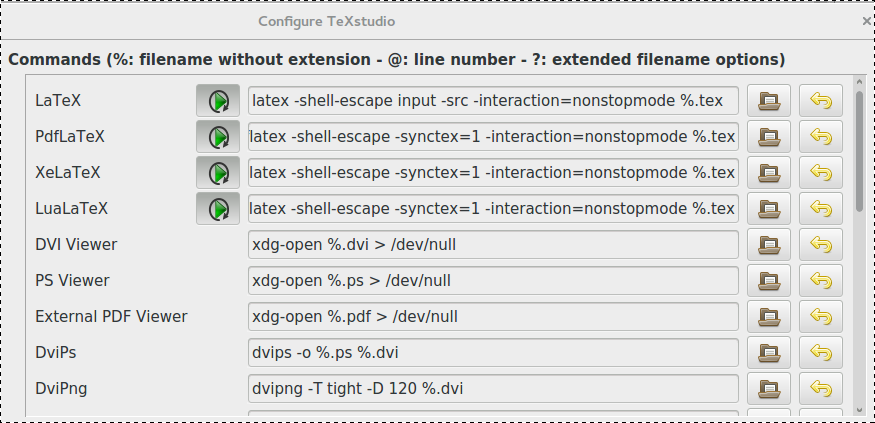
\includegraphics[width=0.75\textwidth]{figures/TeXstudio}
\caption{Configure \tex{}studio}
\label{ch_1_texstudio_config}
\end{figure}

%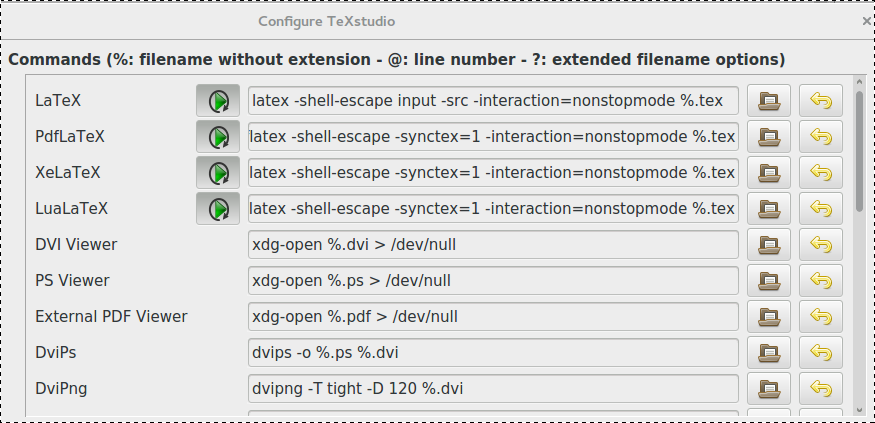
\includegraphics[width=0.75\textwidth]{figures/TeXstudio}

If you are interested in using \latex to display \emph{bash} code, take a look at the \emph{packages.tex} document in the \textsl{settings} folder of the source documents on my \emph{GitHub} site. In the \emph{packages.tex} document there is a \emph{\textbackslash{}lset\{\}} block of code.\footnote{I apologize to the author but I do not recall where I found the block of code.} It is this code that formats the \emph{lstlisting} package that displays the \emph{bash} code. It was this code that allowed me to dispense with the \emph{minted} package.

\add{Add a chapter illustrating the differences between minted and lstlisting.}

\section{\latex and dynamic links}

Since this document is typeset using \latex, you will find many hyperlinks embedded through out the document. I try to clearly identify hyperlinks, but the only true indication that text is a hyperlink is when you hover the mouse over text that is colored, the mouse icon changes from a pointer to a small hand. The hyperlink may be to an external source such as an Internet Webpage or the hyperlink may be to another part of the document.

\section{Where's the meat and potatoes?}

If you don't like reading code, you may not find this book all that appetising. I use lots of comments in my code. In a way, the \emph{comments} are the \emph{Meat and Potatoes}. You will also see that I am a big fan of manpages. I consider the manpages as the \emph{gravy}. I am sure that I will annoy you with my repeated attempts to encourage you to read manpages. Actually, the manpages are just a subset of the documentation that is available to help you learn about Linux commands. \textit{You will not get your \emph{dessert} unless you read the documentation!}

\section{Punctuation} 

Writing about code presents several challenges to the goal of writing with clarity. For example, some Linux commands can be used as verbs. How should one distinguish between the regular use of the command and the verb use of the command? I have chosen the following conventions:

\begin{itemize}
	\item \tbi{Double quotations ""} I surround string names with the double quotation.
	\item \tbi{Single upright quotation \textquotesingle{}\textquotesingle{}} I use single upright quotations to highlight commands with command options. Alternatively, I sometimes place a command with options unquoted after a colon.
	\item \tbi{\emph{Emphasis}}  I use \emph{emphasis} to highlight Linux commands, software names, usernames, etc.
	\item \tbi{Lists of commands} If I list several commands in a row after a colon, I will not put use emphasis.
	\item \tbi {Bold-italic} To highlight a command, I sometimes use bold-italic.
	\item \tbi{Italics} If I have a suggestion for you, if I recommend that you test something, I will put the recommendation in \textit{italics}.
	\item \tbi{Caps} Technical terms that are ubiquitous and always written in caps are left in caps, unless I choose to put them in bold-italic for emphasis.
	\item \tbi{Slanted text} I use slanted text for pathnames \textsl{/home/myhome/myfolder}.
	\item \tbi{Keywords} I use the \latex \keyword{keyword} font to highlight \emph{keywords} such as a command like \keyword{mkdir}. I then build an index of the keywords that are listed at the end of this book.
\end{itemize}

\section{Who do you think you are?}

As per the little flag in the header of this document, I am proudly Canadian-eh. After high-school, without the high, I toiled purposely and industriously at University. Upon graduation, I worked on the high seas of accountancy\footnote{\href{https://www.youtube.com/watch?v=7YUiBBltOg4}{Monty Python's Meaning of Life}}, moved on to being a cultured madman\footnote{\href{http://www.penguin.com/static/html/classics/readingguides/deptfordtrilogy.php}{RobertsonDavies - Deptford Trilogy}}, and then finally careened towards IT. I have expired certifications in: A+, Microsloth MCSE 2000/2003, Cisco CCNP, CIISP, and GSEC.

I began my IT career working for a small IT consulting company. For 2 years, I did everything from laying CAT 5 wiring and setting up LANs to hosting websites and email on a FreeBSD server. This is when I began working with Linux. Next, I worked for a large oil-field services company as a Senior Systems Analyst contributing to environmental degradation and global warming. I spent most of my time with Cisco and other network vendor's gear managing LANs within the company's WAN. Guilt about my role in contributing to the slow death of our planet began to override my drive for financial gain and I chose to find alternate employ. For the past several years, I have worked again as a Senior Systems Analyst, this time for a manufacturer of energy saving products supporting a mixed Microsoft-Linux environment.

In my spare time, I read British and Canadian history, paddle a SUP, run long distances, cycle (and re-cycle), and ballroom dance with my wife. As you will notice, I use the metric system\footnote{\href{http://www.joeydevilla.com/2008/08/13/countries-that-dont-use-the-metric-system/}{Metric makes sense unless you have twelve fingers.}}, the British spelling system (unless typesetting \latex and creating man pages), and the Oxford and.

One of my favourite quotes that I think adequately sums up the human condition is the following: \tbi{Time flies like an arrow, fruit flies like a banana.}

\section{More context}

The type of Linux support that I provide at work is fairly limited. Here is a not-complete list of the type of Linux-related tasks that I work on...

\begin{itemize}
	\item \tbi{Building virtual servers for the user community: } I get requests from various departments to build specific-purpose Linux servers. I build the servers on an open source host. The Linux flavour depends on user preference. Some users like Ubuntu, some Debian, some Centos, some Fedora.
	\item \tbi{Building and managing virtual servers for System Administration: } Our DNS, SQL, internal web, and network monitoring servers are Linux-based.
	\item \tbi{Supporting manufacturing team: }The manufacturing team use Linux workstations in various stages of the manufacturing process. The tools are fairly sophisticated and run only on Linux.
	\item \tbi{Supporting Linux users: } Linux users tend to be fairly independent and able, so the type of support tends to be at a higher level than basic support. I typically deal with issues related to: setting up Samba shares, Git connections to software repositories, setting up Virtual Machines, SSH connectivity, permissions and ACLs, Apache and Wordpress configurations, Linux package configurations, etc.
\end{itemize}

As previously stated, at home, I alternate between using a Fedora 23 box and a MacBook Pro laptop, depending upon where I want to work. If it is warm and sunny on the deck and the beer is cold, I have no choice but to use the MBP laptop. With the Fedora 23 box, my home folder is on a separate partition from the root drive. On an irregular basis, I backup my home folder with rsync (a manual process). Occasionally, I shut my system down and use \href{http://clonezilla.org/downloads.php}{Clonezilla} to image my hard drive to a second hard drive. I have been able to mostly ween myself from the Microsoft bosom. The exceptions are few and are all related to software vendors who refuse to provide a Linux alternative. In order to deal with these exceptions, I built a couple of Windoze VMs using \href{http://virt-manager.ort}{Virtual Machine Manager} and launch these whenever I have to use the proprietary software...which thankfully is rarely.

\section{What's it all about Murray?}
\label{sec:allabout}

This book is principally about one thing: working at the command line using Linux builtin commands and \href{http://www.gnu.org/software/coreutils/coreutils.html}{GNU Coreutils}. If you become proficient at the command line, you will have mastered an important piece of becoming a Linux System Administrator. Since, I wrote this book using the \latex typesetting system, the title has become: \tbi{Writing about Linux System Administration using \latex}.

Like most things, the more you dig into them and play around, the more you learn. I am a proponent of \tbi{RTFM}\textit{\tbi{ - Read The Funky Manual} and don't think that someone will simply give you all the answers to your questions so that you don't have to expend any effort at all}.

This book has a very exploratory approach. You will find that I present code in a step-by-step manner supported by a lot of comments. I issue a command and maybe it doesn't work. I then try another command. Along the way, I attempt to describe my reasoning and methodology.

\tbi{Disclaimer:}

\begin{addmargin}[1em]{2em}
\textit{I am very old. I have a lot of memories, clutter, and useless pieces of information stuck between my ears. I simply cannot retain all the diverse bits of code and jetsam that are in my brain that I find useful. Just a sec, is it my brain that is useful or are the bits of information useful? Better get rid of the danglies\footnote{\href{http://blog.oxforddictionaries.com/2011/09/participles-how-not-to-dangle/}{Oxford Dictionaries to the rescue}} and rewrite this sentence. I simply cannot retain all the useful and diverse bits of code and jetsam that clutter the inside of my brain.}
\end{addmargin}

In order to address this issue of running out of brain disk space, I began documenting my Linux System Administration adventures using notebooks and binders and simple digital text documents. Much later, I switched to using \href{https://evernote.com}{Evernote}. Evernote is fairly useful for brain dumping information and creating folder hierarchy, but it is a pain to search and organize your information. Evernote refuses to create a Linux package for its product.\footnote{\href{https://www.youtube.com/watch?v=eGKdle1bbvo}{The company should also feel shame.}} However, there is a pretty good Linux alternative called \href{http://sourceforge.net/projects/nevernote/}{NixNote} which is what I use on my Fedora 23 system. For some reason, I cannot copy a webpage clip into NixNote. I can copy it as unformatted text, but if I try to copy it directly, I get a sync error. Instead, I have to use Evernote's Web Client in order to copy a webpage into my Evernote repository. I can then sync this cloud version of Evernote from the NixNote client.

Consequently, I wanted to move my notes from Evernote to a digital book form that had these features: indexing, table of contents, a professional look, sophisticated search capability, ease of revision, and a well-supported open source community behind it. Enter \latex! What a wonderful adventure this has been! Not only am I sharpening my Linux skills, but in the process I am developing a new skill, typesetting with \latex. My first motivation to use \latex came when I started a couple of \href{https://en.wikipedia.org/wiki/Massive\_open\_online\_course}{MOOCs}. The first was Coursera's \href{https://www.coursera.org/course/scicomp}{High Performance Scientific Computing} offered by the University of Washington's \href{http://faculty.washington.edu/rjl/}{Dr. Randall J. LeVeque}. \textit{If you want to improve your understanding of Linux and Python and you like math, take this course.} The other course was an EdX course,  \href{https://www.edx.org/course/introduction-solar-systems-astronomy-asux-ast111x-0}{Introduction to Solar Systems Astronomy}. I audited both courses. To help in retaining content, I wanted ready access to my notes, comments, and explorations that were typeset, especially important with the EdX course since it used many complex differential equations. This is where LaTeX excels...typesetting scientific and mathematical formulae.

And, finally, one topic that Dr. LeVeque covered in the HPSC course was \href{https://github.com/}{GitHub}.  Dr. LeVeque's discussions on \keyword{GitHub} helped me position this book as a collaborative project so that others can download it and contribute to its improvement.

I started this book in the early winter 2015 and finished the first published version in the fall of 2016.

\section{What this book is not about!}

This book is not a brain dump that can be used to easily challenge the current Linux certification exams. The book may help you get a base understanding of Linux System Administration tasks, but your study or reading of this book will not on its own help you succeed in passing these exams. In fact, when you check the curriculum for each certification, you will see that there are many gaps in the knowledge base that I present in this book. Here is a URL list of the main organizations that provide Linux certifications.

\begin{enumerate}
\item{\href{https://training.linuxfoundation.org/certification/lfcs}{Linux Foundation Certified System Administrator}}
\item{\href{https://www.lpi.org/certification/}{Linux Professional Institute}}
\item{\href{https://www.redhat.com/en/services/certification}{Red Hat Certification}}
\end{enumerate}

\section{\href{http://www.poetryfoundation.org/poem/171647}{Beware the Jabberwok, my son!}}

\textit{Trust nothing that I have written! Find alternative explanations! Verify everything and test all commands! Do not simply memorize a command, make sure it works.} This warning is especially applicable to non-Fedora-system users. Will the commands that I present work on a Debian or BSD system? The code will more likely work best on Fedora, CentOS, and RHEL systems.

My style of writing and the quality of my writing will undoubtedly displease some, cause bad gas and foul odours, but so be it. This book on Linux System Administration is a compilation of my investigation to understand the  Linux command line. Each time I check and edit my notes, I seem to come across syntax and coding errors and discover further insights. I have endeavoured to present code and information that is error free, but there is no guarantee that I have eliminated all errururs. I encourage you to point out errors and to make suggestions. If you only want to heap scorn on me, censure me, and build a wall of unkindness, I suggest that you join a political party that aligns with your sensibilities.\\

This book may become a living document for the next couple of years as long as my energies and interest remain high, that is, as long as red wine remains affordable and beer remains cold.

\howto{Latex - How to make list of all URLs?}





